\documentclass[../main.tex]{subfiles}
\setcounter{chapter}{2}

\begin{document}

    \chapter{Linear Block Codes}

    \section{Hamming weight, Minimum Distance and Code Rate}
    The Hamming weight $w_H(x)$ of a codeword or vector $x$ is defined as the amount of non-zero elements or vector coordinates, which ranges from zero to length $n$ of said codeword.

    \begin{equation*}
        w_H(x) = \sum_{j=0}^{n-1} w_H(x_j), \text{ where } w_H(x_j) =
        \begin{cases}
            0, &\text{if } x_j = 0 \\
            1, &\text{if } x_j \neq 0
        \end{cases}
    \end{equation*}

    \noindent
    The Hamming distance $d_H(x,y)$ between two codewords or vectors $x$ and $y$ is defined as amount of elements or coordinates where $x$ and $y$ differ.

    \begin{equation*}
        d_H(x,y) = \sum_{j=0}^{n-1} w_H(x_j+y_j), \text{ where } w_H(x_j+y_j) =
        \begin{cases}
            0, \text{if } x_j=y_j \\
            1, \text{if } x_j \neq y_j
        \end{cases}
    \end{equation*}

    \begin{equation*}
        d_H(x,y) =  w_H(x,y)
    \end{equation*}

    \noindent
    The minimum distance $d_min$ of code $C$ is the minimum distance between two different codewords. The minimum distance for linear codes is equal to the minimum weight \autocite{bossert1999channel}. However, a codeword containing only zeros and therefore having a distance of zero is disregarded as the minimum distance cannot be zero.


    Let $x,y$ be codewords in code $C$. A received vector, which is the sent vector $x$ in $C$, plus error vector $e$ can only be corrected if the distance between any other codeword $y$ in $C$ fulfill

    \begin{equation*}
        d_{min}(x, x+e) < d_{min}(y, x+e) \text{ or } w_{min}(e) < w_{min}(x+y+e).
    \end{equation*}

    \noindent
    Therefore

    \begin{equation*}
         w_{min}(e) \leq \frac{d-1}{2},
    \end{equation*}

    \noindent
    where $d$ is the distance. This is written as

    \begin{equation*}
        t \leq \frac{d-1}{2} \text{ or } d \geq 2t+1,
    \end{equation*}

    \noindent
    where $t$ is the amount of errors that can be corrected.

    In general, a code $C$ of length $n$, with $M$ codewords, and a minimum distance $d=d(C)$, is called an $(n,M,d)$ code. Then M$ \leq q^{n-d+1}$ and the coderate of a $q$-ary $(n,M,d)$ code is at most $1-\frac{d-1}{n}$.

    A linear $q$-ary code of lenght $n$, with $k$ codewords or message symbols, and distance $d$ is called a $(n,k,d)$ code or $(n,k)$ code. The code rate is defined as

    \begin{equation*}
        R=\frac{log_qk}{n}.
    \end{equation*}

    \noindent
    If, according to Shannon's channel coding theorem, rate $R$ is less than capacity $C$, then the code exists but if rate $R$ is larger than capacity $C$, the error probability is 1 and the length of the codeword becomes infinite.


    \section{Singleton Bound}
    It is preferable to have a large minimum distance $d$ so that many errors can be corrected. Also, a large amount of codewords $M$ would allow for efficient use of bandwidth when transmitting over a noisy channel. Unfortunately, increasing $d$ tends to increase $n$ or decrease $M$. The Singleton bound is an upper bound for $M$ in terms of $n$ and $d$. A code that satisfies the Singleton bound is called a MDS code (maximum distance separable). The Singleton bound can be written as

    \begin{equation*}
        q^d \leq \frac{q^{n+1}}{M}
    \end{equation*}

    \noindent
    for the MDS code to obtain the largest possible value of $d$ for a given $n$ and $M$. Reed-Solomon codes are an important class of MDS codes \autocite{trappe2006introduction}.


    \section{Maximum-likelihood Decoding}
    There are two principles of decoding. In hard-decision decoding the received bits are believed to be either 1 or 0 in binary transmission. The decoding is done bit by bit. In soft-decision decoding, the received codewords may contain samples of bits with many values, not just 1 or 0. Calculating the closest error-free codeword is more complicated but soft-decision decoding has better performance than the hard-decision decoding.

    Assuming hard-decision decoding is used, the received codeword is decoded into its closest codeword measured by its smallest Hamming distance. This minimum probability of error principle is called Maximum-Likelihood or Minimum Distance Decoding \autocite{geisel1990tutorial}.

    The model of the binary symmetric channel (BSC) \autocite{mackay2003information} in \Cref{fig:binary_symmetric_channel} shows that the channel has binary input and output with an error probability, the channel is characterised by the following conditions if $c$ is the transmitted code and $r$ the received code:

    \begin{align*}
        \begin{rcases*}
            P(r=0|c=0) &= 1-p\\
            P(r=0|c=1) &= p\\
            P(r=1|c=0) &= p\\
            P(r=1|c=1) &= 1-p
        \end{rcases*} \text{ and } 0 \leq p \leq \frac{1}{2}\\
    \end{align*}

    Comparing all received codewords $r$ to all transmitted codewords $c$ as a direct way of correcting errors would not be inefficient. This means storing all $2k$ code vectors and performing equally as many comparisons for each received codeword, resulting in error vectors of which the vector with the smallest distance is probably the transmitted codeword. A more practical decoding method would be Syndrome decoding which will be described in \Cref{sec:syndrome_decoding}.


    \section{Hamming Codes}

    \begin{figure}[htp]
        \centering
        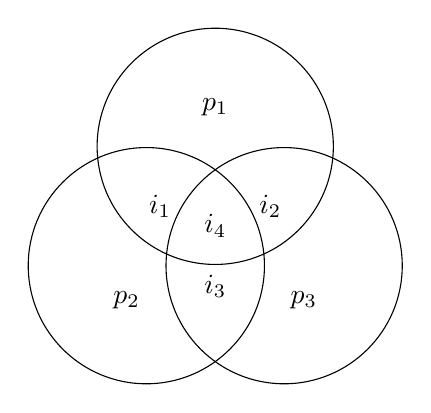
\begin{tikzpicture}[
                set/.style = {draw, circle, minimum size=3cm, align=center},
            ]
            \node (A) at (0,0) [set] {}; \node at (90:0.5cm) {$p_1$};
            \node (B) at (240:1.75cm) [set] {}; \node at (240:2.25cm) {$p_2$};
            \node (C) at (300:1.75cm) [set] {}; \node at (300:2.25cm) {$p_3$};

            \node at (barycentric cs:A=1,B=1) [left] {$i_1$};
            \node at (barycentric cs:A=1,C=1) [right] {$i_2$};
            \node at (barycentric cs:B=1,C=1) [below] {$i_3$};
            \node at (barycentric cs:A=1,B=1,C=1) [] {$i_4$};
        \end{tikzpicture}
        \caption{Relation between information and parity bits}
        \label{fig:information_and_parity_bits}
    \end{figure}

    \begin{figure}[htp]
        \centering
        \begin{tikzpicture}[
                            > = latex,
                node distance = 7mm,
                   box/.style = {draw, minimum size=10mm},
                   dot/.style = {circle, draw, fill, minimum size=1mm, inner sep=0mm, node contents={}},
            ]
            % data word nodes
            \node (di1) [box] at (0,0) {$i_1$};
            \node (di2) [box] at (0,-1) {$i_2$};
            \node (di3) [box] at (0,-2) {$i_3$};
            \node (di4) [box] at (0,-3) {$i_4$};

            % code word nodes
            \node (ci1) [box] at (10,0) {$i_1$};
            \node (ci2) [box] at (10,-1) {$i_2$};
            \node (ci3) [box] at (10,-2) {$i_3$};
            \node (ci4) [box] at (10,-3) {$i_4$};
            \node (cp1) [box] at (10,-4) {$p_1$};
            \node (cp2) [box] at (10,-5) {$p_2$};
            \node (cp3) [box] at (10,-6) {$p_3$};

            % mod 2 adder nodes
            \node (a1) [box] at (5,-4) {$i_1+i_2+i_4$};
            \node (a2) [box] at (5,-5.5) {$i_1+i_3+i_4$};
            \node (a3) [box] at (5,-7) {$i_2+i_3+i_4$};

            % connection nodes
            \node (n1) [dot, right=0.5cm of di1];
            \node (n2) [dot, right=1cm of di2];
            \node (n3) [dot, right=1.5cm of di3];
            \node (n4) [dot, right=2cm of di4];
            \node (n5) [left=1cm of cp2] {};
            \node (n6) [left=0.5cm of cp3] {};

            % connections
            \draw (di1) edge (n1); \draw[->] (n1) edge (ci1);
            \draw (di2) edge (n2); \draw[->] (n2) edge (ci2);
            \draw (di3) edge (n3); \draw[->] (n3) edge (ci3);
            \draw (di4) edge (n4); \draw[->] (n4) edge (ci4);
            % i1
            \draw[->] (n1) |- node[dot] {} (a1.south west);
            \draw[->] (n1) |- (a2.south west);
            % i2
            \draw[->] (n2) |- node[dot] {} (a1.west);
            \draw[->] (n2) |- (a3.south west);
            % i3
            \draw[->] (n3) |- node[dot] {} (a2.west);
            \draw[->] (n3) |- (a3.west);
            % i4
            \draw[->] (n4) |- node[dot] {} (a1.north west);
            \draw[->] (n4) |- node[dot] {} (a2.north west);
            \draw[->] (n4) |- (a3.north west);
            % p1
            \draw[->] (a1.east) -- (cp1.west);
            % p2
            \draw[->] (a2.east) -| (n5.center) (n5.center) |- (cp2.west);
            % p3
            \draw[->] (a3.east) -| (n6.center) (n6.center) |- (cp3.west);

            % legends
            \coordinate[above=0.25cm of di1, label={4-bit data word}];
            \coordinate[above=0.25cm of ci1, label={7-bit code word}];
            \coordinate[below=0.5cm of a3, label={modulo 2 adders}];
        \end{tikzpicture}
        \caption{ Hamming (7,4) encoder.}
        \label{fig:hamming_encoder}
    \end{figure}

    \begin{figure}[htp]
        \centering
        \begin{tikzpicture}[
                        > = latex,
            node distance = 7mm,
                box/.style = {draw, minimum size=10mm},
                dot/.style = {circle, draw, fill, minimum size=1mm, inner sep=0mm, node contents={}},
                sum/.style = {circle, draw, minimum size=6mm,
                            path picture={\draw[thick,shorten <=1.5mm,shorten >=1.5mm,-]
                                            (\ppbb.north) edge (\ppbb.south)
                                            (\ppbb.west)  edge (\ppbb.east);
                                            },% end of path picture /node content/
                            node contents={}},
            ]
            % code word nodes
            % data word nodes
            % mod 2 adder nodes
            % error correction nodes
            % connection nodes
            % connections
            % legends
        \end{tikzpicture}
        \caption{ Hamming (7,4) decoder.}
        \label{fig:hamming_decoder}
    \end{figure}


    \section{Syndrome Decoding} \label{sec:syndrome_decoding}


    \section{Cyclic Codes}


    \section{BCH Codes}


    \section{Generating BCH Code}


    \section{Decoding BCH Code}


\end{document}



